\title{Tendon Robot Statics}
\author{John Till}
\date{}

\documentclass[12pt]{article}

\usepackage[a4paper, margin=0.75in]{geometry}
\usepackage[colorlinks=true,urlcolor=blue]{hyperref}
\usepackage{amsmath,amssymb}
\usepackage{graphicx}

\usepackage{xcolor}
\definecolor{OffWhite}{rgb}{0.93,0.93,0.93}
\definecolor{QtCommentColor}{rgb}{0,0.5,0}
\definecolor{QtKeywordColor}{rgb}{0.5,0.5,0}
\definecolor{QtPurpleColor}{rgb}{0.5,0,0.5}
\definecolor{QtGlobal}{rgb}{0.808,0.361,0}
\definecolor{QtFunctionColor}{rgb}{0,0.404,0.486}
\definecolor{BlenderPythonString}{rgb}{0.392,0,0}
\definecolor{BlenderPythonKeyword}{rgb}{0.502,0,0.314}
\definecolor{BlenderPythonGold}{rgb}{0.373,0.373,0}
\definecolor{BlenderPythonLiteral}{rgb}{0,0,0.784}
\definecolor{BlenderPythonBackground}{rgb}{0.6,0.6,0.6}

\usepackage[T1]{fontenc} %for upquotes in listings
\usepackage{textcomp} %for upquotes in listings
\usepackage{listings}
\lstset{
		language=C++,
		escapeinside={!-}{-!},
		upquote=true,
		%
		otherkeywords={Vector3d, DiagonalMatrix, VectorXd, Matrix3d, Map, MatrixXd, Vector6d, Vector4d,
		              Matrix6d, Eigen, Upper, std, fstream, Matrix3Xd,
									UnitX, pow, inverse, transpose, segment, data, UnitZ, cross, hat_squared,
									hat_postmultiply, hat_premultiply,
									Zero, Identity, UnitY, cosseratTendonRobotOde, ode4, cols, row, main, shootingFunction,
									block, rotation_error, solveLevenbergMarquardt, toDenseMatrix,
									selfadjointView, llt, close, kirchhoffTendonRobotOde, cwiseProduct, cwiseMin,
									cwiseMax, getRouting, normalized},
    morekeywords=[2]{Vector3d, DiagonalMatrix, VectorXd, Matrix3d, Map, MatrixXd, Vector6d, Vector4d,
		                 Matrix6d, Eigen, Upper, std, fstream, Matrix3Xd},
		morekeywords=[3]{UnitX, UnitZ, pow, inverse, transpose, segment, data, cross, hat_squared,
		                 hat_postmultiply, hat_premultiply,
		                 Zero, Identity, UnitY, cosseratTendonRobotOde, ode4, cols, row, main, shootingFunction,
										 block, rotation_error, solveLevenbergMarquardt, toDenseMatrix,
										 selfadjointView, llt, close, kirchhoffTendonRobotOde, cwiseProduct, cwiseMin,
										 cwiseMax, getRouting, normalized},
    %
		frame = single,
		rulecolor=\color{black},
    tabsize=4, % tab space width
    showstringspaces=false, % don't mark spaces in strings
		%
		basicstyle=\footnotesize,%\color{QtIdentifier},
		backgroundcolor=\color{OffWhite},
    commentstyle=\color{QtCommentColor}, % comment color
    keywordstyle=\color{QtKeywordColor}, % keyword color
		keywordstyle=[2]{\color{QtPurpleColor}},
		keywordstyle=[3]{\color{QtFunctionColor}},
    stringstyle=\color{QtCommentColor} % string color
}

\begin{document}

\makeatletter
\renewcommand{\@maketitle}{
\newpage
\null
\vskip 2em
\begin{center}
{\LARGE \@title \par}
\end{center}
\par
} \makeatother

\maketitle

\section{Tendon Robot Model in C++}

This example shows how to implement the tendon robot model from the paper \href{https://ieeexplore.ieee.org/document/5957337}{``Statics and Dynamics of Continuum Robots With General Tendon Routing and External Loading''}, which is also described in Chapter 4 of the dissertation \href{https://etd.library.vanderbilt.edu//available/etd-10042011-115347/}{``The Mechanics of Continuum Robots: Model-based Sensing and Control''}.

At the top of the C++ script, we start with the simple independent parameters:
\begin{lstlisting}
//Independent Parameters
const double E = 200e9;
const double G = 80e9;
const double rad = 0.001;
const double rho = 8000;
const Vector3d g = 9.81*Vector3d::UnitX();
const double L = 0.5;
const int num_tendons = 4;
\end{lstlisting}
These are straightforward. However, the independent parameters also include the tendon routing paths. The journal paper considers general routing paths with offsets given by the functions $\boldsymbol{r}_i(s)$ for $1 \leq i \leq$ num\_tendons, as well as derivatives $\dot{\boldsymbol{r}}_i(s)$ and $\ddot{\boldsymbol{r}}_i(s)$. Tendons are often routed parallel to the backbone, and simulations involving functions as design parameters tend to be a bit complicated, so for now we'll assume there is no dependence on $s$ so that $\boldsymbol{r}_i$ is constant. We implement this in C++ for four tendons spaced $90^\circ$ apart:
\begin{lstlisting}
const double tendon_offset = 0.01506;
#define R(theta) (tendon_offset*Vector3d(!-\textcolor{QtFunctionColor}{cos}-!(theta), !-\textcolor{QtFunctionColor}{sin}-!(theta), 0))
const Vector3d r[num_tendons] = {R(0), R(pi/2), R(pi), R(pi*3/2)};
#undef R
\end{lstlisting}
We define a macro function ``R'' which makes it easier to initialize the array ``r'' with vectors spaced $90^\circ$ apart. We immediately undefine the macro so that we can use the symbol ``R'' in the future without accidently invoking the macro. Now there is just one more independent parameter; the input to the forward kinematics problem is the tension in each tendon:
\begin{lstlisting}
const VectorXd tau = Vector4d(15,0,0,0);
\end{lstlisting}
We set $\tau_1 = 15$N and $\tau_2 = \tau_3 = \tau_4 = 0$N.
With the independent parameters set, there are several dependent parameter calculations:
\begin{lstlisting}
//Dependent parameter calculations
const double area = pi*pow(rad,2);
const double I = pi*pow(rad,4)/4;
const double J = 2*I;
const DiagonalMatrix<double, 3> Kse (G*area,G*area,E*area);
const DiagonalMatrix<double, 3> Kbt (E*I,E*I,G*J);
const Matrix3d Kse_dense = Kse.toDenseMatrix();
const Matrix3d Kbt_dense = Kbt.toDenseMatrix();
\end{lstlisting}
There is some redundancy in the stiffness matrices; we have both dense and diagonal data structures so that we can use either representation without making a conversion.

The core of the model is the ODE function. The state variables are $\boldsymbol{p}$, $\boldsymbol{R}$, $\boldsymbol{v}$, and $\boldsymbol{u}$. At the start of the ODE function we unpack the state vector:
\newpage
\begin{lstlisting}
void cosseratTendonRobotOde(VectorXd& y_s_out, VectorXd& y){
    //Unpack state vector
    Matrix3d R = Map<Matrix3d>(&y[3]);
    Vector3d v = Map<Vector3d>(&y[12]);
    Vector3d u = Map<Vector3d>(&y[15]);
\end{lstlisting}
The paper describes how one must solve a linear system to find $\dot{\boldsymbol{v}}$ and $\dot{\boldsymbol{u}}$. We declare the variables to setup this system:
\begin{lstlisting}
Vector3d a = Vector3d::Zero();
Vector3d b = Vector3d::Zero();
Matrix3d A_plus_Kse = Kse_dense; = Kse_dense;
Matrix3d G = Matrix3d::Zero();
Matrix3d H_plus_Kbt = Kbt_dense;
\end{lstlisting}
In Equation (16) of the paper, the left-hand side coefficient matrix is given by
\begin{align*}
\begin{bmatrix}
\boldsymbol{K}_{se} + \boldsymbol{A} & \boldsymbol{G} \\ \boldsymbol{G}^T & \boldsymbol{K}_{bt} + \boldsymbol{H}
\end{bmatrix}.
\end{align*}
For the program, it makes sense to roll $\boldsymbol{K}_{se} + \boldsymbol{A}$ into a single variable, and likewise for $\boldsymbol{K}_{bt} + \boldsymbol{H}$. Then we sum the variables as described just before Equation (15):
\begin{lstlisting}
for(int i = 0; i < num_tendons; i++){
    Vector3d pb_si = u.cross(r[i]) + v;
    double pb_s_norm = pb_si.!-\textcolor{QtFunctionColor}{norm}-!();
    Matrix3d A_i = -hat_squared(pb_si)*(tau(i)/pow(pb_s_norm,3));
    Matrix3d G_i = -hat_postmultiply(A_i,r[i]);
    Vector3d a_i = A_i*(u.cross(pb_si));

    a += a_i;
    b += r[i].cross(a_i);
    A_plus_Kse += A_i;
    G += G_i;
    H_plus_Kbt += hat_premultiply(r[i],G_i);
}
\end{lstlisting}
After the summation in this loop, the variables will have the correct values. The smaller components are combined to setup the linear system coefficient matrix:
\begin{lstlisting}
Matrix6d K;
K << A_plus_Kse, G, G.transpose(), H_plus_Kbt;
\end{lstlisting}
The right-hand side ``rhs'' is given just before Equation (16), and we construct the vector:
\begin{lstlisting}
Vector3d nb = Kse*(v - Vector3d::UnitZ());
Vector3d mb = Kbt*u;

Vector6d rhs;
rhs << -u.cross(nb) - !-\textcolor{QtFunctionColor}{transposeMultiply}-!(R,rho*area*g) - a,
       -u.cross(mb) - v.cross(nb) - b;
\end{lstlisting}
We solve for the body frame internal force and moment as intermediate variables before setting the right-hand side values. This is partially to recognize physically relevant terms, but also to avoid repeated calculations of ``nb''.

\newpage \noindent
With the linear system setup, we are positioned to complete the ODE function by solving for the derivatives:
\begin{lstlisting}
    //Pack state vector derivative
    Map<Vector3d> p_s(&y_s_out[0]);
    Map<Matrix3d> R_s(&y_s_out[3]);
    Map<Vector6d> vs_and_us(&y_s_out[12]);

    //ODEs
    p_s = R*v;
    R_s = hat_postmultiply(R,u);
    vs_and_us = K.selfadjointView<Eigen::Upper>().llt().!-\textcolor{QtFunctionColor}{solve}-!(rhs);
}
\end{lstlisting}
One of Eigen's linear solvers is used to solve the 6x6 linear system. The ``selfadjointView'' takes advantage of the symmetry of ``K''.

After the ODE function, we move on to the shooting method's objective function. At the top of the function we unpack the guess:
\begin{lstlisting}
static MatrixXd Y; //Declare Y global to save results
VectorXd shootingFunction(VectorXd guess){
    Vector3d n0 = guess.segment<3>(0);
    Vector3d v0 = Kse.inverse()*n0 + Vector3d::UnitZ();
    Vector3d u0 = guess.segment<3>(3);
\end{lstlisting}
One of the unknown state variables is $\boldsymbol{v}(0)$, but we guess $\boldsymbol{n}(0)$ and solve for $\boldsymbol{v}(0)$ since I suspect this will lead to better \emph{numerical conditioning} of the objective function. Next we integrate the tendon robot ODE:
\begin{lstlisting}
VectorXd y0(18);
y0 << p0, Map<VectorXd>(Matrix3d(R0).data(), 9), v0, u0;

//Numerically integrate the Cosserat rod equations
Y = ode4<cosseratTendonRobotOde>(y0, L);
\end{lstlisting}
Once the integration is done, we can find the violation of the static equilibrium equations. There are forces acting on the final disk from the backbone and tendon attachment points. We extract the internal force in the backbone:
\begin{lstlisting}
//Find the internal forces in the backbone prior to the final plate
Vector3d vL = Y.block<3,1>(12,Y.cols()-1);
Vector3d uL = Y.block<3,1>(15,Y.cols()-1);

Vector3d nb = Kse*(vL - Vector3d::UnitZ());
Vector3d mb = Kbt*uL;
\end{lstlisting}
Then we sum the forces and moments acting on the plate, starting with the backbone, then looping over the tendons:
\begin{lstlisting}
//Find the equilibrium error at the tip, considering tendon forces
Vector3d force_error = -nb;
Vector3d moment_error = -mb;
for(int i = 0; i < num_tendons; i++){
    Vector3d pb_si = uL.cross(r[i]) + vL;
    Vector3d Fb_i = -tau(i)*pb_si.normalized();
    force_error += Fb_i;
    moment_error += r[i].cross(Fb_i);
}
\end{lstlisting}
The tendon loading terms are given by Equations (18), (19), and (20). Finally we complete the objective function by returning a single error vector:
\begin{lstlisting}
    Vector6d distal_error;
    distal_error << force_error, moment_error;

    return distal_error;
}
\end{lstlisting}

With the objective function complete, we are finally ready to write the simulation driver. Over in the main function, the problem is solved in just a few lines:
\begin{lstlisting}
int main(int, char**){
    Vector6d init_guess = Vector6d::Zero(); //nb and u

    //Solve with shooting method
    VectorXd wrench_soln = solveLevenbergMarquardt<shootingFunction>
                               (init_guess, 1e-12, 500, 1e-2, 0.5, 1e-7, 1e-9);
\end{lstlisting}
The solver uses finite differences to build the Jacobian, and the default finite difference increments are too small. Thus we specify all the parameters for the ``solveLevenbergMarquardt'' function to use larger increments. With the problem solved, the results should be visualized. I think it can be difficult to understand tendon robot behavior from simple line plots, so we'll generate a render of the robot instead. The backbone curve, tendon curves, and full pose at nine points along the backbone are saved to text files:
\begin{lstlisting}
    //Save results for Blender visualization
    std::fstream file("centerline.dat", std::fstream::out);
    file << Y.block(0,0,3,Y.cols());
    file.close();

    MatrixXd tendonlines(3*num_tendons, Y.cols());
    for(int i = 0; i < Y.cols(); i++){
        Vector3d p = Y.block<3,1>(0,i);
        Matrix3d R = Map<Matrix3d>(&Y(3,i));
        for(int j = 0; j < num_tendons; j++)
            tendonlines.block<3,1>(3*j,i) = p + R*r[j];
    }
    file = std::fstream("tendonlines.dat", std::fstream::out);
    file << tendonlines;
    file.close();
		
    const int num_disks = 9;
    Matrix3Xd disks(3,4*num_disks);
    for(int i = 1; i <= num_disks; i++){
        int j = ((Y.cols()-1) * i) / num_disks;
        Vector3d p = Y.block<3,1>(0,j);
        Matrix3d R = Map<Matrix3d>(&Y(3,j));
        disks.block<3,3>(0,4*(i-1)) = R;
        disks.block<3,1>(0,4*(i-1)+3) = p;
    }
    file = std::fstream("disks.dat", std::fstream::out);
    file << disks;
    file.close();

    return 0;
}
\end{lstlisting}
Running the C++ script should produce three files ``centerline.dat'', ``tendonlines.dat'', and ``disk.dat''. These files will be located in the active directory the program is run from, which by default is a build folder when using Qt.

\section{Visualization with Blender}

One of the nice features of Blender is that in addition to using the user interface, you can also perform modeling tasks using Python scripts. This is perfect for generating 3d models from simulation results.

The output text files should be moved to the Blender subfolder. The Python script to render the tendon robot is contained in ``Tendon\_Robot\_Render.blend''. Upon opening the file with Blender, the Python scripting pane will be in the upper left. There is a ``Run Script'' button on the bottom right of the pane as shown below:
\begin{figure}[h]
	\centering
		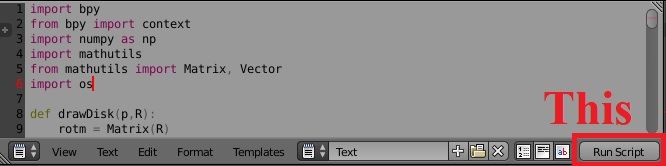
\includegraphics[width=0.95\textwidth]{fig/ScriptingPane.jpg}
	\label{fig:Pane}
\end{figure}

\noindent
Running this script with the text files present will cause a render of the robot to be saved to the ``output'' subfolder:
\begin{figure}[h]
	\centering
		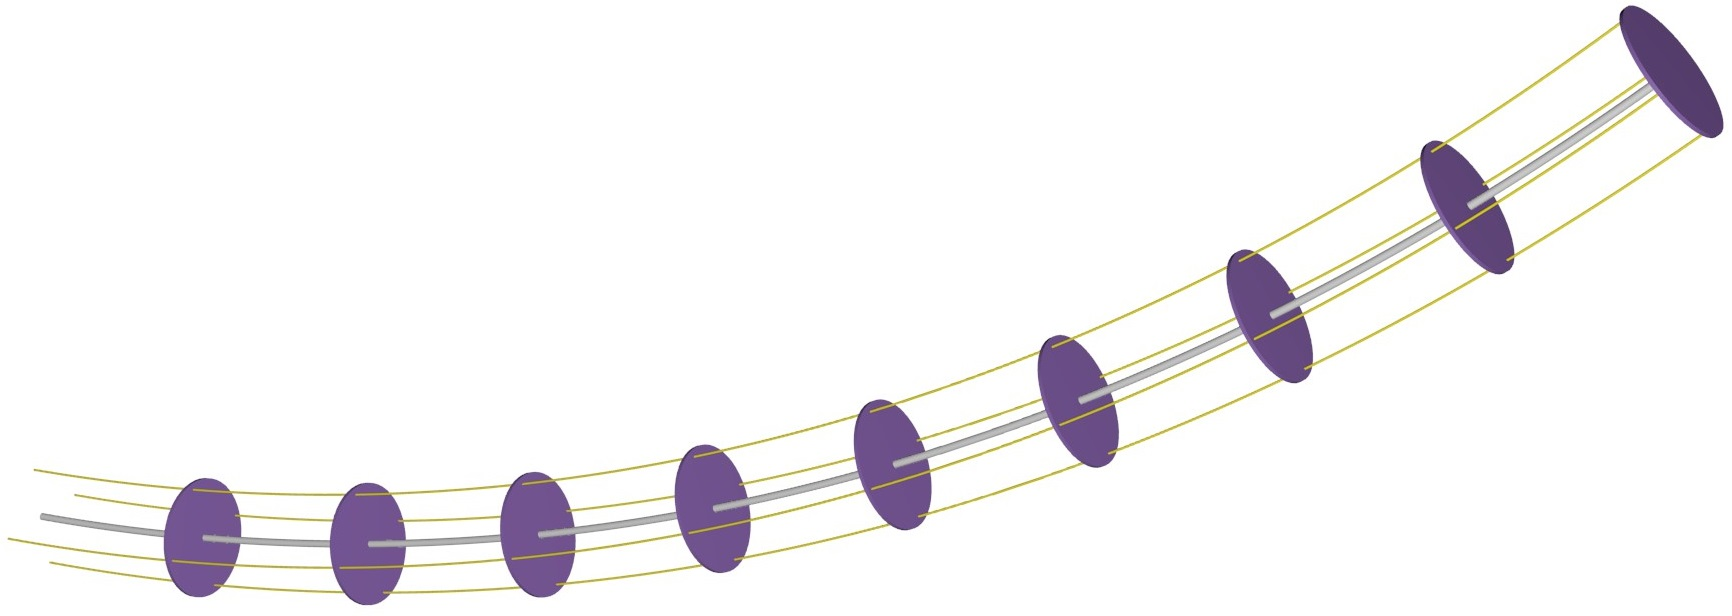
\includegraphics[width=0.8\textwidth]{fig/TendonRobotRender.jpg}
\end{figure}

\noindent Applying a tension on the first tendon has caused the backbone to bend, exactly as we would expect. Since the distributed weight of the backbone is not very large, the backbone curve nearly has a constant curvature.

\lstset{
		language=Python,
		escapeinside={!-}{-!},
		%
		deletekeywords={def, type, object, range, len, int},
		otherkeywords={def, True, False, type, object, range, len},
		morekeywords=[2]{def},
		morekeywords=[3]{True, False, type, object, range, len},
		%
		frame = single,
		rulecolor=\color{black},
    tabsize=4, % tab space width
    showstringspaces=false, % don't mark spaces in strings
		%
		basicstyle=\footnotesize,%\color{QtIdentifier},
		%backgroundcolor=\color{BlenderPythonBackground},
    %commentstyle=\color{QtCommentColor}, % comment color
    keywordstyle=\color{BlenderPythonKeyword}, % keyword color
		keywordstyle=[2]{\color{BlenderPythonGold}},
		keywordstyle=[3]{\color{BlenderPythonLiteral}},
    stringstyle=\color{BlenderPythonString}, % string color
		literate={0}{{\textcolor{BlenderPythonLiteral}{0}}}{1}%
             {1}{{\textcolor{BlenderPythonLiteral}{1}}}{1}%
             {2}{{\textcolor{BlenderPythonLiteral}{2}}}{1}%
             {3}{{\textcolor{BlenderPythonLiteral}{3}}}{1}%
             {4}{{\textcolor{BlenderPythonLiteral}{4}}}{1}%
             {5}{{\textcolor{BlenderPythonLiteral}{5}}}{1}%
             {6}{{\textcolor{BlenderPythonLiteral}{6}}}{1}%
             {7}{{\textcolor{BlenderPythonLiteral}{7}}}{1}%
             {8}{{\textcolor{BlenderPythonLiteral}{8}}}{1}%
             {9}{{\textcolor{BlenderPythonLiteral}{9}}}{1}%
             {.0}{{\textcolor{BlenderPythonLiteral}{.0}}}{2}% Following is to ensure that only periods
             {.1}{{\textcolor{BlenderPythonLiteral}{.1}}}{2}% followed by a digit are changed.
             {.2}{{\textcolor{BlenderPythonLiteral}{.2}}}{2}%
             {.3}{{\textcolor{BlenderPythonLiteral}{.3}}}{2}%
             {.4}{{\textcolor{BlenderPythonLiteral}{.4}}}{2}%
             {.5}{{\textcolor{BlenderPythonLiteral}{.5}}}{2}%
             {.6}{{\textcolor{BlenderPythonLiteral}{.6}}}{2}%
             {.7}{{\textcolor{BlenderPythonLiteral}{.7}}}{2}%
             {.8}{{\textcolor{BlenderPythonLiteral}{.8}}}{2}%
             {.9}{{\textcolor{BlenderPythonLiteral}{.9}}}{2}%
						 {type}{type}{4}%
						 {object}{object}{6}%
						 {range}{range}{5}%
						 {len}{len}{3}%
						 {int}{int}{3}%
						 {format}{format}{6}%
}

We won't get into the details of the different parts of the Blender Python script here. The script is given in whole below to close out the example:
\begin{lstlisting}
import bpy
from bpy import context
import numpy as np
import mathutils
from mathutils import Matrix, Vector
import os

def drawDisk(p,R):
    rotm = Matrix(R)
    (x_base, y_base, z_base) = Vector(p) + rotm * Vector((0, 0, -0.001/2))
    (x_top, y_top, z_top) = Vector(p) + rotm * Vector((0, 0, 0.001/2))
    	
    #Curve settings
    curveData = bpy.data.curves.new('myCurve', type='CURVE')
    curveData.dimensions = '!-\textcolor{BlenderPythonString}{3D}-!'
    curveData.resolution_u = 2
    polyline = curveData.splines.new('POLY')
    polyline.points.add(1)
    polyline.points[0].co = (x_base, y_base, z_base, 1)
    polyline.points[1].co = (x_top, y_top, z_top, 1)

    cross_section = bpy.ops.curve.primitive_bezier_circle_add(radius=0.017)
    ob = bpy.context.object
    ob.name = 'cross_section_disk'

    curveOB = bpy.data.objects.new('myCurve', curveData)
    scn = bpy.context.scene
    scn.objects.link(curveOB)
    scn.objects.active = curveOB
    curveOB.select = True
    curveOB.data.bevel_object = bpy.data.objects['cross_section_disk']
    curveOB.data.use_fill_caps = True
    
    mat = bpy.data.materials.new("RGBA")
    mat.use_transparency = True;
    mat.diffuse_color = (79/255.0, 41/255.0, 132/255.0)
    mat.alpha = 1;
    curveOB.active_material = mat

def drawRod(p):
    (rows,cols) = p.shape

    #Curve settings
    curveData = bpy.data.curves.new('tCurve', type='CURVE')
    curveData.dimensions = '!-\textcolor{BlenderPythonString}{3D}-!'
    curveData.resolution_u = 2
    polyline = curveData.splines.new('POLY')
    polyline.points.add(cols-1)
        
    cross_section = bpy.ops.curve.primitive_bezier_circle_add(radius=0.001)
    ob = bpy.context.object
    ob.name = 'tcross_section'

    #Loop through spatial steps
    for i in range(0,cols):
    	x,y,z = p[0,i], p[1,i], p[2,i]
    	polyline.points[i].co = (x, y, z, 1)
            
    curveOB = bpy.data.objects.new('myCurve', curveData)
    scn = bpy.context.scene
    scn.objects.link(curveOB)
    scn.objects.active = curveOB
    curveOB.select = True
    curveOB.data.bevel_object = bpy.data.objects['tcross_section']
    curveOB.data.use_fill_caps = True
    
def drawTendon(p):
    (rows,cols) = p.shape

    #Curve settings
    curveData = bpy.data.curves.new('tCurve', type='CURVE')
    curveData.dimensions = '!-\textcolor{BlenderPythonString}{3D}-!'
    curveData.resolution_u = 2
    polyline = curveData.splines.new('POLY')
    polyline.points.add(cols-1)
        
    cross_section = bpy.ops.curve.primitive_bezier_circle_add(radius=0.0003)
    ob = bpy.context.object
    ob.name = 'tcross_section_tendon'

    #Loop through spatial steps
    for i in range(0,cols):
    	x,y,z = p[0,i], p[1,i], p[2,i]
    	polyline.points[i].co = (x, y, z, 1)
            
    curveOB = bpy.data.objects.new('myCurve', curveData)
    scn = bpy.context.scene
    scn.objects.link(curveOB)
    scn.objects.active = curveOB
    curveOB.select = True
    curveOB.data.bevel_object = bpy.data.objects['tcross_section_tendon']
    curveOB.data.use_fill_caps = True
    
    mat = bpy.data.materials.new("RGBA")
    mat.use_transparency = True;
    mat.diffuse_color = (255/255.0, 221/255.0, 0)
    mat.alpha = 1;
    curveOB.active_material = mat
    
### MAIN ###
script_dir = os.getcwd() #<-- absolute path of dir the script is in
bpy.context.scene.world.horizon_color = (1,1,1) #white background
scene = bpy.data.scenes["Scene"]
scene.render.resolution_x = 1280*2
scene.render.resolution_y = 720*2

#Load data
centerline = np.loadtxt( os.path.join(script_dir, 'centerline.dat'))
tendonlines = np.loadtxt( os.path.join(script_dir, 'tendonlines.dat'))
disks = np.loadtxt( os.path.join(script_dir, 'disks.dat'))
num_disks = int(disks.shape[1]/4);
num_tendons = int(tendonlines.shape[0]/3);

#Delete objects already in the scene
for item in bpy.data.objects:
    if item.type == 'MESH' or item.type=='CURVE':
        item.select = True
        bpy.ops.object.delete()

#Create the render
drawRod(centerline)
for i in range(0,num_tendons):
    drawTendon(tendonlines[3*i:3*(i+1), 0:tendonlines.shape[1]])
for i in range(0,num_disks):
    drawDisk(disks[0:3,4*i+3], disks[0:3,4*i:4*i+3])

rel_path = 'output/TendonRobotRender.jpg'
abs_file_path = os.path.join(script_dir, rel_path)
bpy.data.scenes["Scene"].render.filepath = abs_file_path
bpy.ops.render.render( animation=False, write_still=True )
\end{lstlisting}

\end{document}